%%%%%%%%%%%%%%%%%%%%%%%%%%%%%%%%%%%%%%%%%%%%%%%%%%%%%%%%%%%%%%%%%%%%%%%%%%%%%%%%
%2345678901234567890123456789012345678901234567890123456789012345678901234567890
%        1         2         3         4         5         6         7         8

\documentclass[letterpaper, 10 pt, conference]{ieeeconf}  % Comment this line out if you need a4paper

%\documentclass[a4paper, 10pt, conference]{ieeeconf}      % Use this line for a4 paper

\IEEEoverridecommandlockouts                              % This command is only needed if 
                                                          % you want to use the \thanks command

\overrideIEEEmargins                                      % Needed to meet printer requirements.

\usepackage[utf8x]{inputenc}
\usepackage{graphicx}
% See the \addtolength command later in the file to balance the column lengths
% on the last page of the document

% The following packages can be found on http:\\www.ctan.org
%\usepackage{graphics} % for pdf, bitmapped graphics files
%\usepackage{epsfig} % for postscript graphics files
%\usepackage{mathptmx} % assumes new font selection scheme installed
%\usepackage{times} % assumes new font selection scheme installed
%\usepackage{amsmath} % assumes amsmath package installed
%\usepackage{amssymb}  % assumes amsmath package installed

\title{\LARGE \bf
Cascading Situation Assessment for Robots
}


\author{Séverin Lemaignan$^{1}$%
\thanks{$^{1}$Séverin Lemaignan is with Centre for Robotics and Neural Systems,
        Plymouth University, Plymouth PL48AA, United Kingdom
        {\tt\small severin.lemaignan@plymouth.ac.uk}}%
}

\usepackage{xspace}
\newcommand{\eg}{e.g.,\xspace}
\newcommand{\etal}{et al.\xspace}
\newcommand{\ie}{i.e.,\xspace}
\newcommand{\etc}{etc.\xspace}
\newcommand{\vs}{vs.\xspace}
\newcommand{\resp}{\textit{resp.}\xspace}
\newcommand{\cf}{cf.\xspace}

\newcommand{\uwds}{{\sc underworlds}\xspace}

\graphicspath{{figs/}}

\usepackage[cache]{minted}
\renewcommand{\theFancyVerbLine}{
  \sffamily\textcolor[rgb]{0.5,0.5,0.5}{\scriptsize\arabic{FancyVerbLine}}}

\newminted{python}{frame=lines,
                    linenos=true,
                    fontsize=\scriptsize,
                    xleftmargin=1.8em}

\newmintinline[python]{python}{fontsize=\footnotesize}

\begin{document}



\maketitle
\thispagestyle{empty}
\pagestyle{empty}


%%%%%%%%%%%%%%%%%%%%%%%%%%%%%%%%%%%%%%%%%%%%%%%%%%%%%%%%%%%%%%%%%%%%%%%%%%%%%%%%
\begin{abstract}

    We introduce hereafter \uwds, a novel framework for \emph{cascading}
    spatio-temporal situation assessment in robotics. \uwds allows programmers
    to represent the robot's environment as real-time distributed data
    structures, containing both scene graphs (for 3D representation of geometries)
    and timelines (for representation of temporal events). \uwds supports
    \emph{cascading} representations: the environment is viewed as a set of
    \emph{worlds} that can each have different spatial and temporal
    granularities, and may depend on each others.
    
    \uwds also provides a set of high-level client libraries and tools to introspect
    and manipulate the environment models.

    This article presents the design and architecture of this open-source tool,
    and explores some applications, along with examples of use.

\end{abstract}


%%%%%%%%%%%%%%%%%%%%%%%%%%%%%%%%%%%%%%%%%%%%%%%%%%%%%%%%%%%%%%%%%%%%%%%%%%%%%%%%
\section{Introduction}


\uwds is a distributed and lightweight framework that enables robot programmers
to build and refine in real-time spatial and temporal models of the environment
surrounding a robot. \uwds makes it easy, then, to share these models amongst
the other software components running on the robot, to eventually provide a
distributed environment model for the robot.

The components which require such spatial and temporal models of the environment
are typically found in the intermediate layers of robotic architectures, between
the low-level perceptual layers, and the high-level decisional layers. They
typically include geometric reasoners (that compute spatial and topological
relations between objects), motion planners, gestures/sequence recognizers.

Difficulties however arise quickly. These different components might need
different models, at different spatial and temporal resolutions. A 3D motion
planner would typically use coarse 3D models of surrounding objects to lower the
computational load while planning, while a spatial reasoner might need on the
contrary a high-resolution model of the environment for accurate rendering when
attempting to estimate the visibility of an object. Spatial models are also
usually large as they might contain a lot of geometric data (including point
clouds and meshes). Efficient sharing of such datasets is non-trivial,
particularly when the said data are dynamically acquired (\eg in the case of
map building or object recognition).

Traditional robotic middlewares like ROS are not particularly well-suited to
deal with these complexities: geometric data can be represented, but are not
first-class citizens (basic tasks like displaying a 3D mesh at a dynamic
position are non-trivial with ROS, for instance) and representing and reasoning
on \emph{alternative states} of the environment is not directly doable.

Representing \emph{alternative states} is actually often critical. For instance,
software components manipulating environment models typically perform better if
the models are physically consistent. However, low-level perception inaccuracies
at the sensor level often introduce hard-to-avoid physical inconsistencies (like
detected objects floating in the air, or on the contrary wrongly inset into
other objects). Therefore, a post-process stage (for instance, using a physics
simulation engine) might be desired to move the objects seen
by the robot into physically-correct positions. Implemented with a classical
approach (for instance, using ROS TF frames), we would get an object {\tt book}
located at the frame {\tt book\_frame}, and a secondary frame {\tt
book\_frame\_corrected} computed by the physics engine. It is easy to see why
such an approach would be quickly confusing (where is in fact my book?) and would not
scale well, with the robot's 3D model cluttered with spurious frames.

Another relevant example pertains to geometric task planning: a geometric task
planner typically need to reason over hypothetical future states of the
environment (``what happen if I move this glass onto that pile of books?'').
The planner might want to quickly generate possible future states, that
themselves might require further processing (for instance, running a physics
simulation). This use-case evidences the need for a flexible representation
system, where models are derived from each others, with partial modifications
and different timescales.



\subsection{Cascading Situation Assessment}

Anchoring perceptions in a symbolic model requires perception abilities and
their symbolic interpretation. We call \emph{physical situation assessment} the
cognitive skill that a robot exhibits when it assesses the nature and content of its
surroundings and monitors its evolution.

Numerous approaches exist, like amodal (in the sense of modality-independent)
\emph{proxies}~\cite{Jacobsson2008}, grounded amodal
representations~\cite{Mavridis2006}, semantic
maps~\cite{Nuechter2008, Galindo2008,Blodow2011} or affordance-based planning
and object classification~\cite{Lorken2008, Varadarajan2011}.

serving a scene from
different viewpoints to compute visibility is not directly possible


\section{Related work}


\cite{sisbot2011situation}
\cite{naef2003blue}
\cite{bustos2016unified}

\uwds is inspired by geometric and temporal reasoning components like {\sc
Spark} (\emph{SPAtial Reasoning \&
Knowledge}~\cite{sisbot2011situation} (see~\cite{lemaignan2016artificial} for a
high-level description of the integration of a component like {\sc Spark} in a
complete robotic architecture).

It acts as a situation assessment reasoner that generates symbolic knowledge from the
geometry of the environment with respect to relations between objects, robots
and humans, also
taking into account the different perspective that each agent has on the
environment.  {\sc Spark} embeds an \emph{amodal} (as defined by Mavridis and
Roy in~\cite{Mavridis2006}: the different perceptual modalities are abstracted
away into a blended spatial model) geometric model of the environment that
serves both as basis for the fusion of the perception modalities and as bridge
with the symbolic layer. This geometric model is built from 3D CAD models of the
objects, furnitures and robots, and full body, rigged models of humans
(Figure~\ref{fig:sparkScreenshot}).  It is updated at run-time by the robot's
sensors (usually, a combination of vision-based tracking of 2D fiducial markers
to identify and localise objects, and Kinect-based skeleton tracking of humans,
optionally assisted by motion capture to accurately track the head motion, which
is required to compute what the human is looking at).

\subsection{Relation to existing robotic middlewares}

\section{Design and Architecture}

\subsection{Cascading architecture}

Figure~\ref{fig|scene} pictures a typically \uwds topology: a graph (that
happens to be a directed acyclic graph on Figure~\ref{fig|scene}, but does not
have to be in the general case -- cycles are permitted) of \emph{clients}
connected through shared data structures called \emph{worlds}.


\begin{figure}
    \centering
    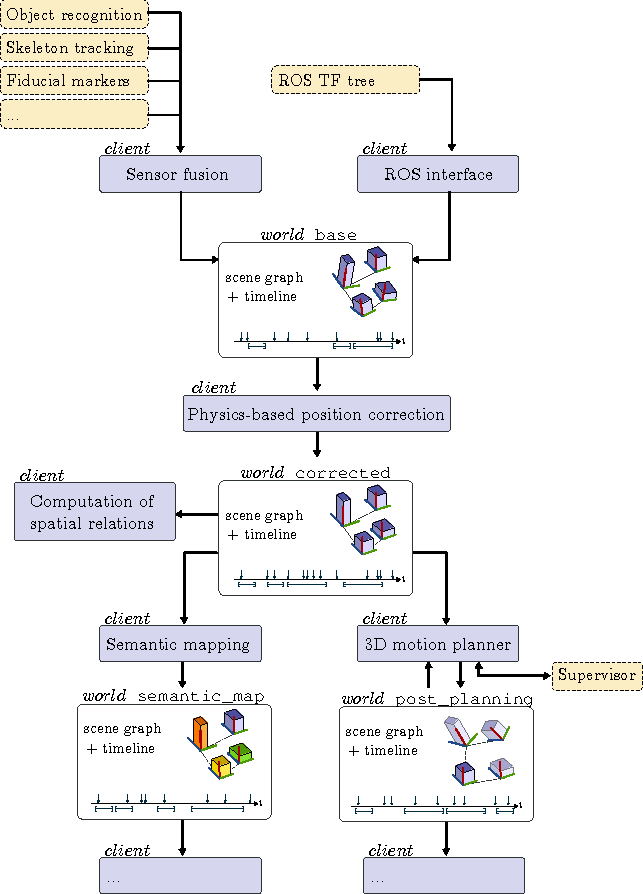
\includegraphics[width=\linewidth]{overview}
    \caption{Schema of a possible \uwds network: eight possible, user-written
    \emph{clients} (in blue) are exchanging environment models through four shared
    \emph{worlds} (made of joint spatial and temporal models). This architecture
    enables successive and modular refinement of the models
    (\emph{cascading} situation assessment), effectively adapted to each
    client's needs (yellow nodes represent other possible components in the system that do not
    interact directly with the \uwds network).}

    \label{fig|scene}

\end{figure}

\subsubsection{Clients}

Software components accessing \uwds worlds are called clients. Some standard
clients (like a 3D visualization tool) are provided with the \uwds package (see
section~\ref{std_clients}), but clients are otherwise written by the end users
using the \uwds client API (see section~\ref{api}).

Clients can both read and write onto the worlds they are connected to, and
automatically see updates broadcasted by other clients connected to the same
worlds.

Four specific types of clients can be distinguished: \textbf{root clients} which
create and update worlds (`write-only' client, like the \emph{Sensor fusion} and
\emph{ROS interface} clients on Figure~\ref{fig|scene}); \textbf{leaf clients}
which on the contrary only read worlds, without modifying them (like the
\emph{Computation of spatial relations} client on Figure~\ref{fig|scene});
\textbf{filters} that copy an input world into an output world, performing
some filtering operation in-between (like the client \textit{Physics-based
position correction}); and \textbf{transformers} which transform one
representation into another (like the \emph{Semantic mapping} client on
Figure~\ref{fig|scene}).

\subsection{Worlds}

Worlds are effectively distributed data structures composed of a scene graph
representing the 3D geometry of the environment, and a timeline storing temporal
events.

Each world is technically independent from every others. Dependencies between
worlds arise from the clients' connections. For instance, filters effectively
create a dependency between worlds. A client like the \textit{Physics-based
position correction} client create a dependency between the world {\tt base} (which
represents here the result of raw sensor fusion) and the world {\tt corrected}
which would be a physically-consistent copy of {\tt base}.
As a result, a \uwds network can be seen as a dependency graph between worlds (where
cyclic dependencies are permissible).

This architecture enables what we call \emph{cascading situation assessment}:
a set of independent software components (the clients) builds and refines
successive models of the environment by a combination of
filtering/transformations steps and model branching.

\subsubsection{Scenes}

\emph{Worlds} contain both a geometric model and a temporal model. The geometric
model is represented as a scene graph. The scene graph has a unique root node,
to which a tree of other nodes is parented.

Nodes in the scene graph have four possible types: \textbf{objects} that represent
concrete physical objects (typically with one or several associated 3D meshes);
\textbf{entities} that represent abstract entities like reference frames or
groups of objects; \textbf{perspectives} that represent viewpoints onto the
scene (like cameras or human gaze); and \textbf{fields} that represent scalar or
vector fields (like the visibility of an object, the working space of robot,
etc. -- note that fields are not yet implemented in the current version of
\uwds, see section~\ref{futurework}).

Every node has a unique ID, a parent, a 3D transformation relative to the parent
and an optional name. \emph{Object} nodes optionally store as well pointers to their
associated meshes.

\subsubsection{Timelines}

\begin{figure}
    \centering
    \includegraphics[width=0.9\linewidth]{timeline}
    \caption{Both events and episodes are stored in the world's \emph{timeline}}

    \label{fig|timeline}
\end{figure}


\subsection{Distributed spatio-temporal models}
\label{arch}

\uwds is not a monolithic piece of software. Instead, it stands for both a
\emph{network of interconnected clients} which manipulate spatial and temporal
models of the robot environment (for instance, a motion planner, a object
detection module, a human skeleton tracker, etc.), and for a {client library}
that makes it easy to interface existing software components with the network.

Critically, the network is essentially hidden to the client: from the user
perspective, the environment model is manipulated as local data structures (the
\emph{worlds}). Modifications to the model are asynchronously synchronised with
a central server (the {\tt underworlded} daemon) and broadcasted to every other
client in the network.

As previously mentioned, worlds are composite data structures comprising of a
scene graph and a timeline. These data structures are synchronized using
Google's gRPC message passing framework\footnote{http://www.grpc.io/}, ensuring
high throughput, reliability, cross-platform/cross-language support. The \uwds
API is specifically discussed hereafter, section~\ref{api}.


\subsubsection*{Performance considerations}

\uwds is meant to broadcast complex environment representations (typically
including large geometric datasets, like meshes) in real-time. \uwds itself does
not perform many CPU intensive tasks (CPU intensive processing tasks -- sensor fusion, physics
simulation, etc. -- are realized by the clients) and as such, the performance
bottleneck is essentially the network's data throughput.

In that regard, one of the simple yet critical optimization performed by \uwds
is automatic caching of mesh data. Mesh data are not transmitted when nodes are
updated; only a hash value of the mesh data. The client can then request the
full data whenever they actually need it.



\section{API \& Clients}

\subsection{API}
\label{api}

As mentioned in section~\ref{arch}, \uwds uses Google's gRPC as message passing
protocol. The protocol is explicitely defined, and bindings to various languages
and platforms can be automatically generated from the protocol definition file
(as of Feb 2017, gRPC can generate bindings for C, C++, C\#, Node.js, PHP, Ruby,
Python, Go and Java on Windows, Mac and Linux).

The cross-platform/cross-language support of gRPC is especially welcomed in the
academic context, as it offers ease and flexibility to plug a variety of
pre-existing components into a \uwds network.


However, the gRPC message passing layer is low-level with respect to the typical
use of \uwds (manipulation of asynchronous, distributed spatio-temporal models
of the robot environment). In particular, the asynchronous fetching (and
conversely, remote updating) of nodes and time-related objects should be
entirely hidden from the user, and managed instead by the \uwds client library.

\uwds currently offers such a high-level client library for Python only. A C++
library is being developed (currently in 'alpha' state).
Listing~\ref{lst|pythonapi} gives a complete example of an \uwds client
performing simple filtering: the client continuously ``listen'' for changes in
an input world, hide some items (in this case, items whose name contain the
string ``{\tt wall}''), and forward all other changes to an output world,
effectively making the output world a copy of the input world with all walls
removed.

\begin{listing}[h!]

\begin{pythoncode}
import underworlds

with underworlds.Context("walls_filter") as ctx:

    in_world = ctx.worlds["example_in"]
    out_world = ctx.worlds["example_out"]

    while True:

        in_world.scene.waitforchanges()

        for node in in_word.scene.nodes:
            if("wall" not in node.name):
                out_world.scene.nodes.update(node)


\end{pythoncode}
    \caption{Example of a simple \uwds Python client named {\tt walls\_filter}:
    the client connects to the \uwds network, efficiently accesses the world
    {\tt example\_in}, filter out some objects, and publish the remaining
    objects in the world {\tt example\_out}.} \label{lst|pythonapi}
\end{listing}

\subsection{Standard Clients}
\label{std_clients}

\subsubsection{3D Visualization}

Interestingly, while \uwds deals with 3D geometries and scenes, it does
represent 3D entities purely as data structures: no visual representation is
involved (and as such, the \uwds server and core libraries do not depend on any
graphics library like OpenGL). However, for all practical purposes, the ability
to visualize the content of a scene is desirable. \uwds provides a standard
client, {\tt uwds view}, that performs real-time 3D rendering of the scene,
using OpenGL (Figure~\ref{fig|uwds-view}).

\begin{figure}
    \centering
    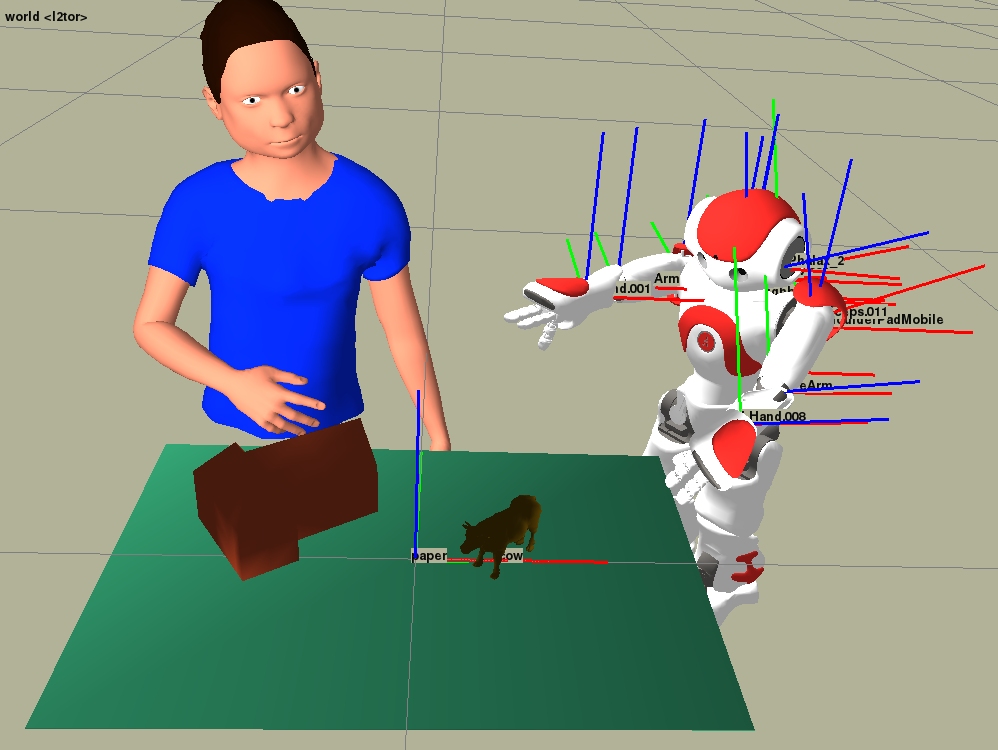
\includegraphics[width=0.9\linewidth]{uwds-screenshot}
    \caption{Screenshot of the {\tt uwds view} 3D visualization and manipulation
    tool.}
    \label{fig|uwds-view}
\end{figure}

This tool also support basic object manipulations, that are broadcasted to the
other \uwds clients as expected.

\subsubsection{Assets loading}

{\tt uwds load}

\subsubsection{Introspection and debugging}

{\tt uwds ls}
{\tt uwds show}

{\tt uwds explorer}


\subsubsection{Interface with ROS}

{\tt uwds tf}

\subsection{Spatial Reasoning}

Spatial reasoning~\cite{O'Keefe1999} is a field in its own right, and has been
used for natural language processing for applications such as direction
recognition ~\cite{Kollar2010,Matuszek2010} or language
grounding~\cite{Tellex2010}.~\cite{Skubic2004} present a spatial reasoner
integrated in a robot which computes symbolic positions of objects.

\begin{figure}
    \centering
    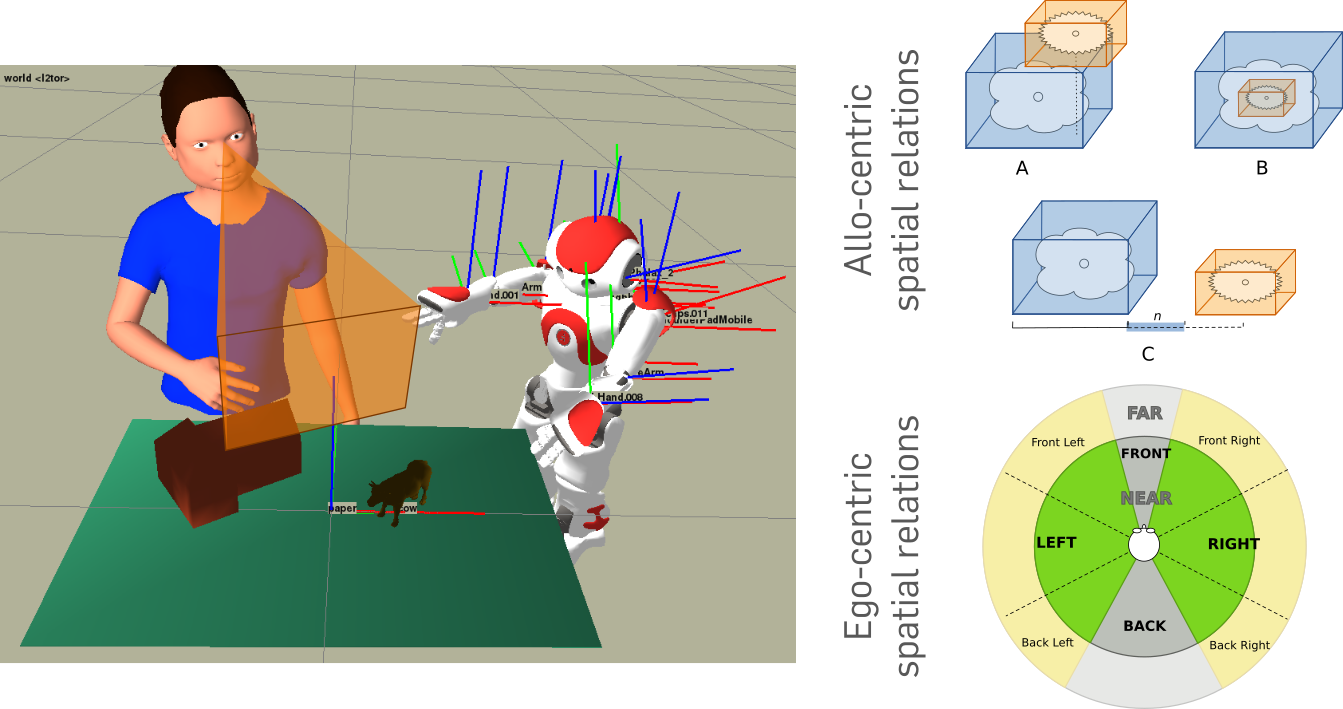
\includegraphics[width=0.9\linewidth]{spatialrelations}
    \caption{The {\tt spatial\_relations} client computes perspective-aware
    spatial relations between objects and agents}
    \label{fig|spatialrelations}
\end{figure}

\cite{Ros2010}

\subsubsection{Visibility computation}

{\tt uwds visibility}

\subsubsection{Perspective Taking}


\section{Application Example}

\begin{figure}
    \centering
    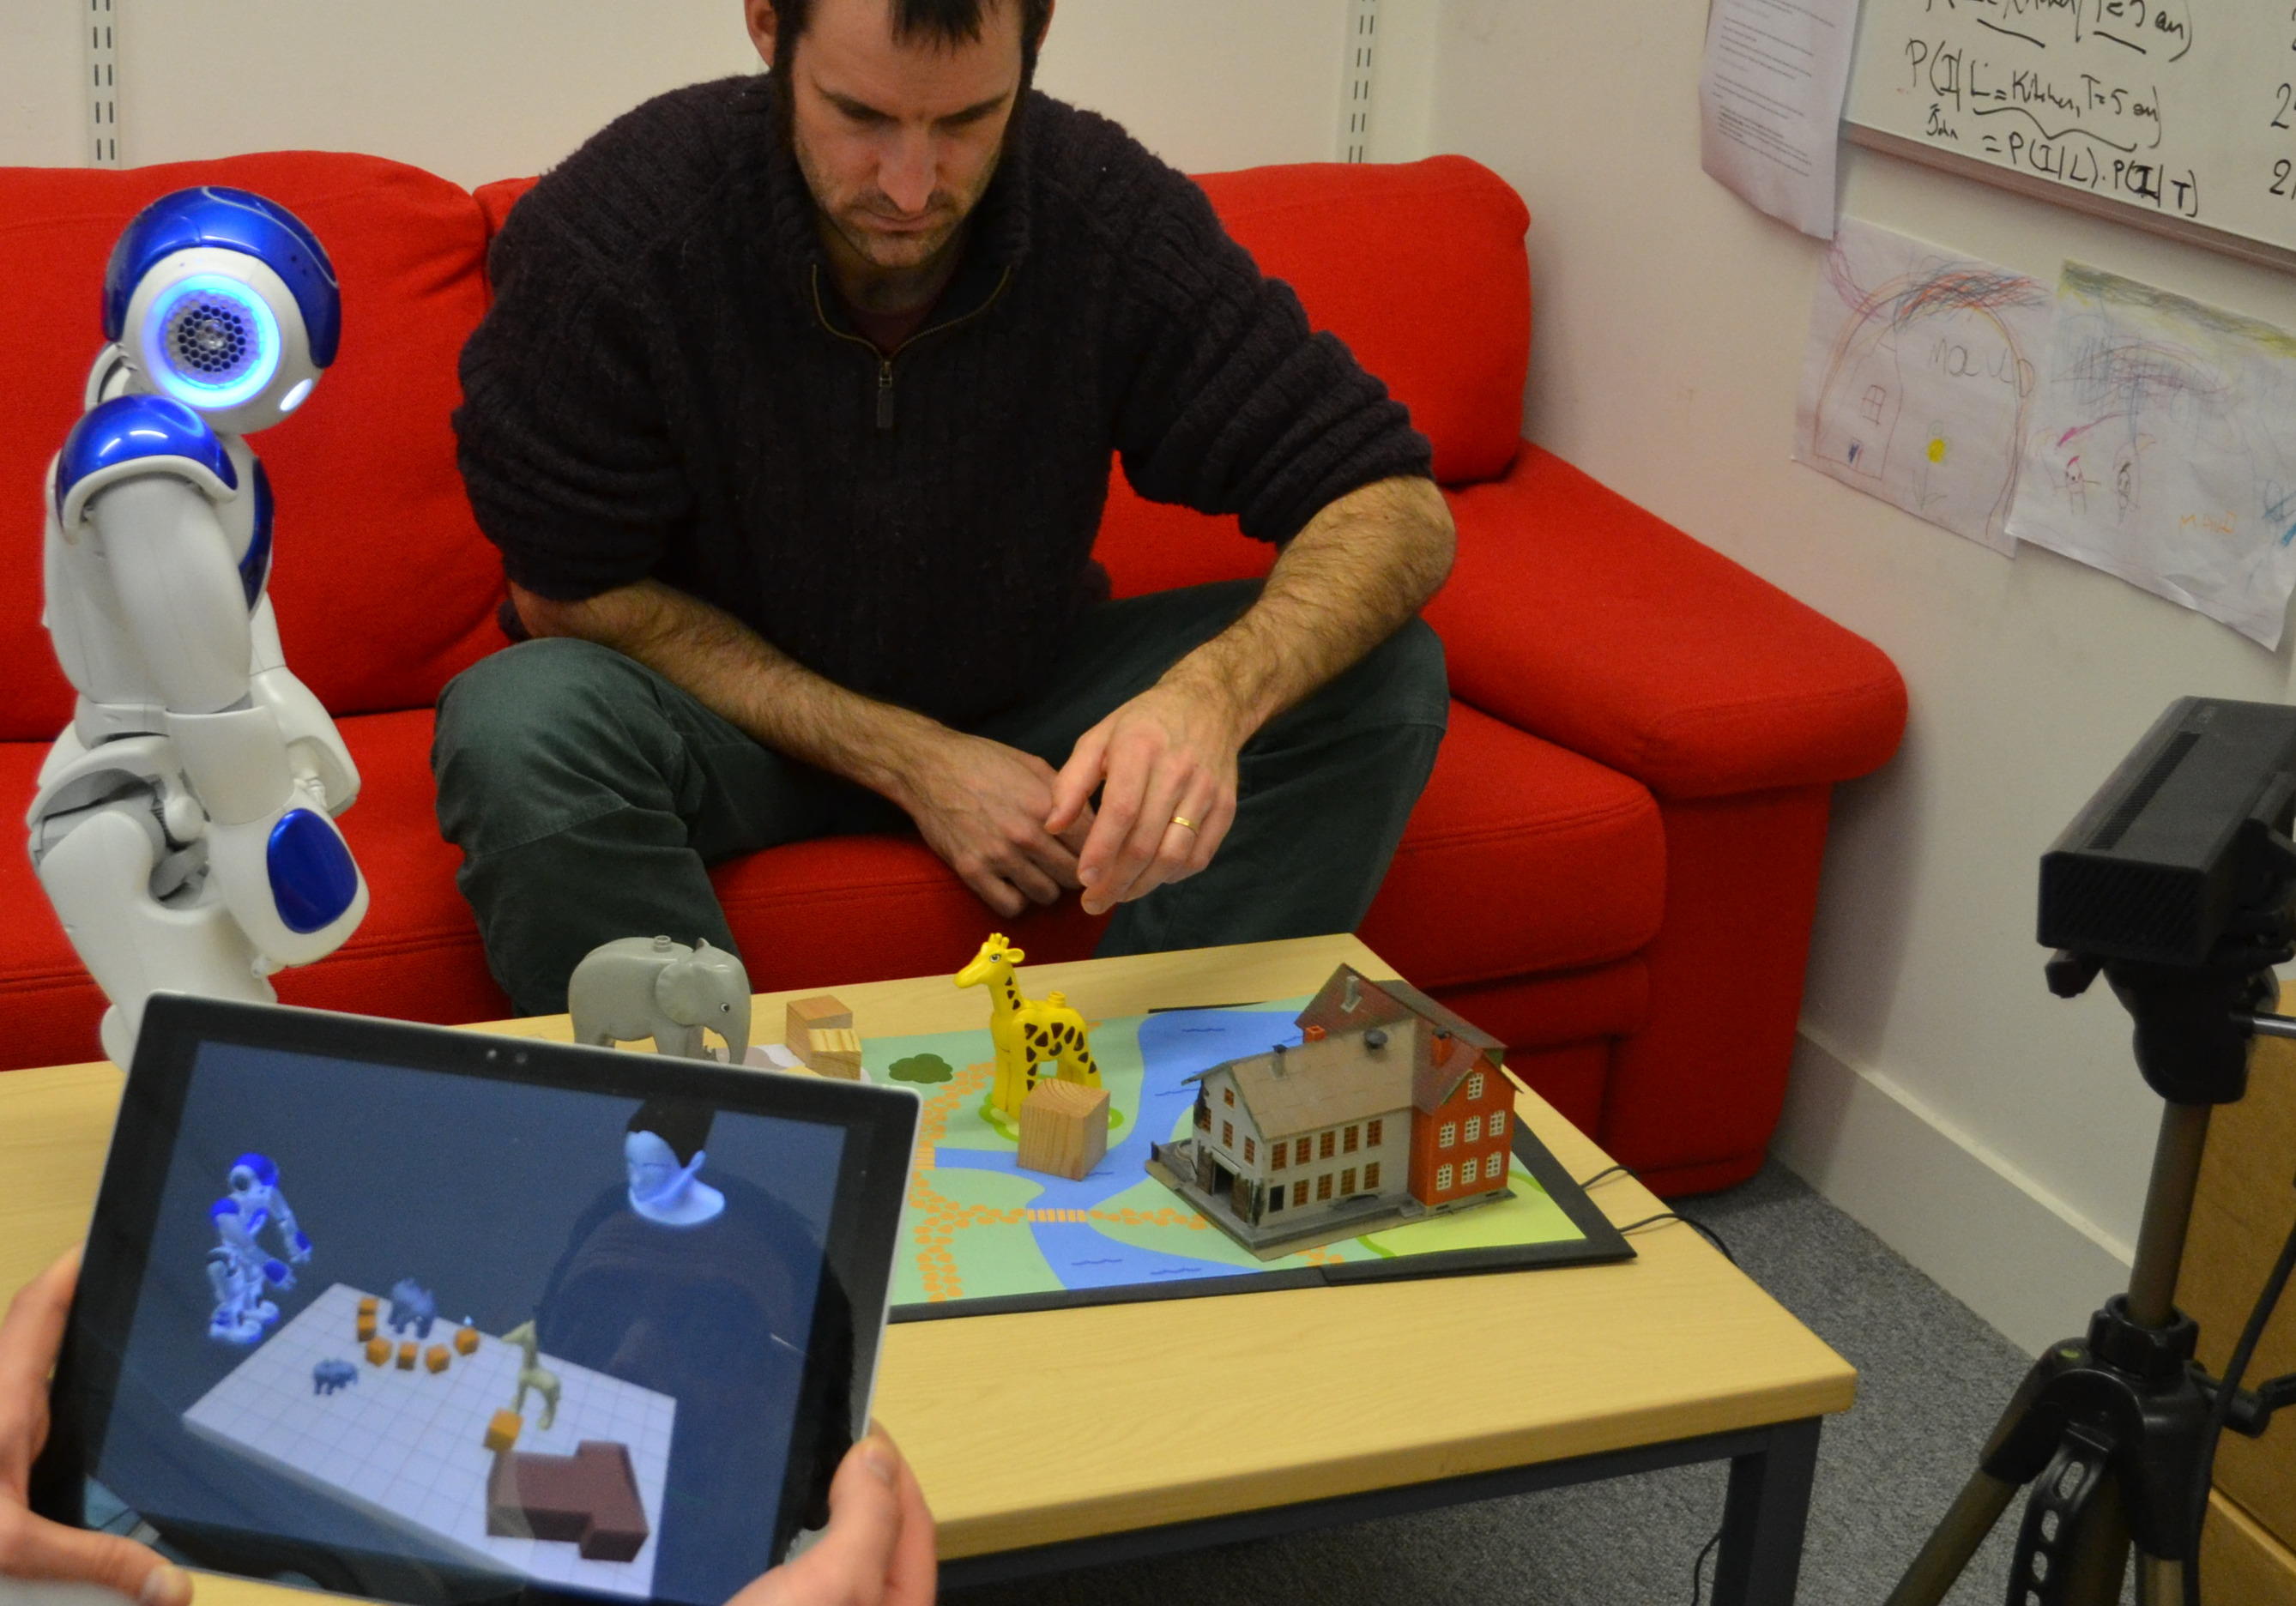
\includegraphics[width=\linewidth]{l2tor-photo2}
    \caption{A user manipulating objects on RFID mat while an operator monitors the interaction via an {\tt uwds view} client}
    \label{fig|l2torexample}
\end{figure}
\uwds has been used within the European L2TOR project~\cite{L2TOR} to implement 

...context + picture

...needs for spatial representation

\subsection*{Architecture}
The scenario consists of a number of \uwds clients that communicate with each other in order to provide an updated virtual representation to the operator. As seen in Figure \ref{fig|l2torexample}, the user interacts with some     
\begin{figure}
    \centering
    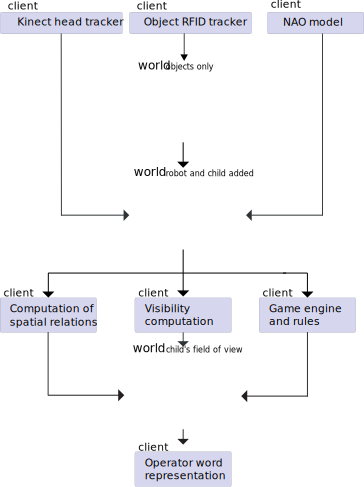
\includegraphics[width=\linewidth]{l2tor-timeline}
    \caption{Schema of the \uwds architecture used in L2TOR project pilot study. }
    \label{fig|l2torarchitecture}
\end{figure}
...diagram with the various \uwds clients

\section{Conclusion}

\subsection{Future work}
\label{futurework}

Representation of fields

Client libraries in more languages

\section*{Acknowledgment}

This work has been supported by the EU H2020 Marie Sk\l odowska-Curie Actions
project DoRoThy (grant 657227) and the EU H2020 L2TOR project (grant 688014).


\bibliographystyle{IEEEtran}
\bibliography{bibliography}




\end{document}
